\chapter{Graphene}
\label{theory}

\section{Graphene}


\begin{wrapfigure}{r}{0.38\textwidth}
  \centering
  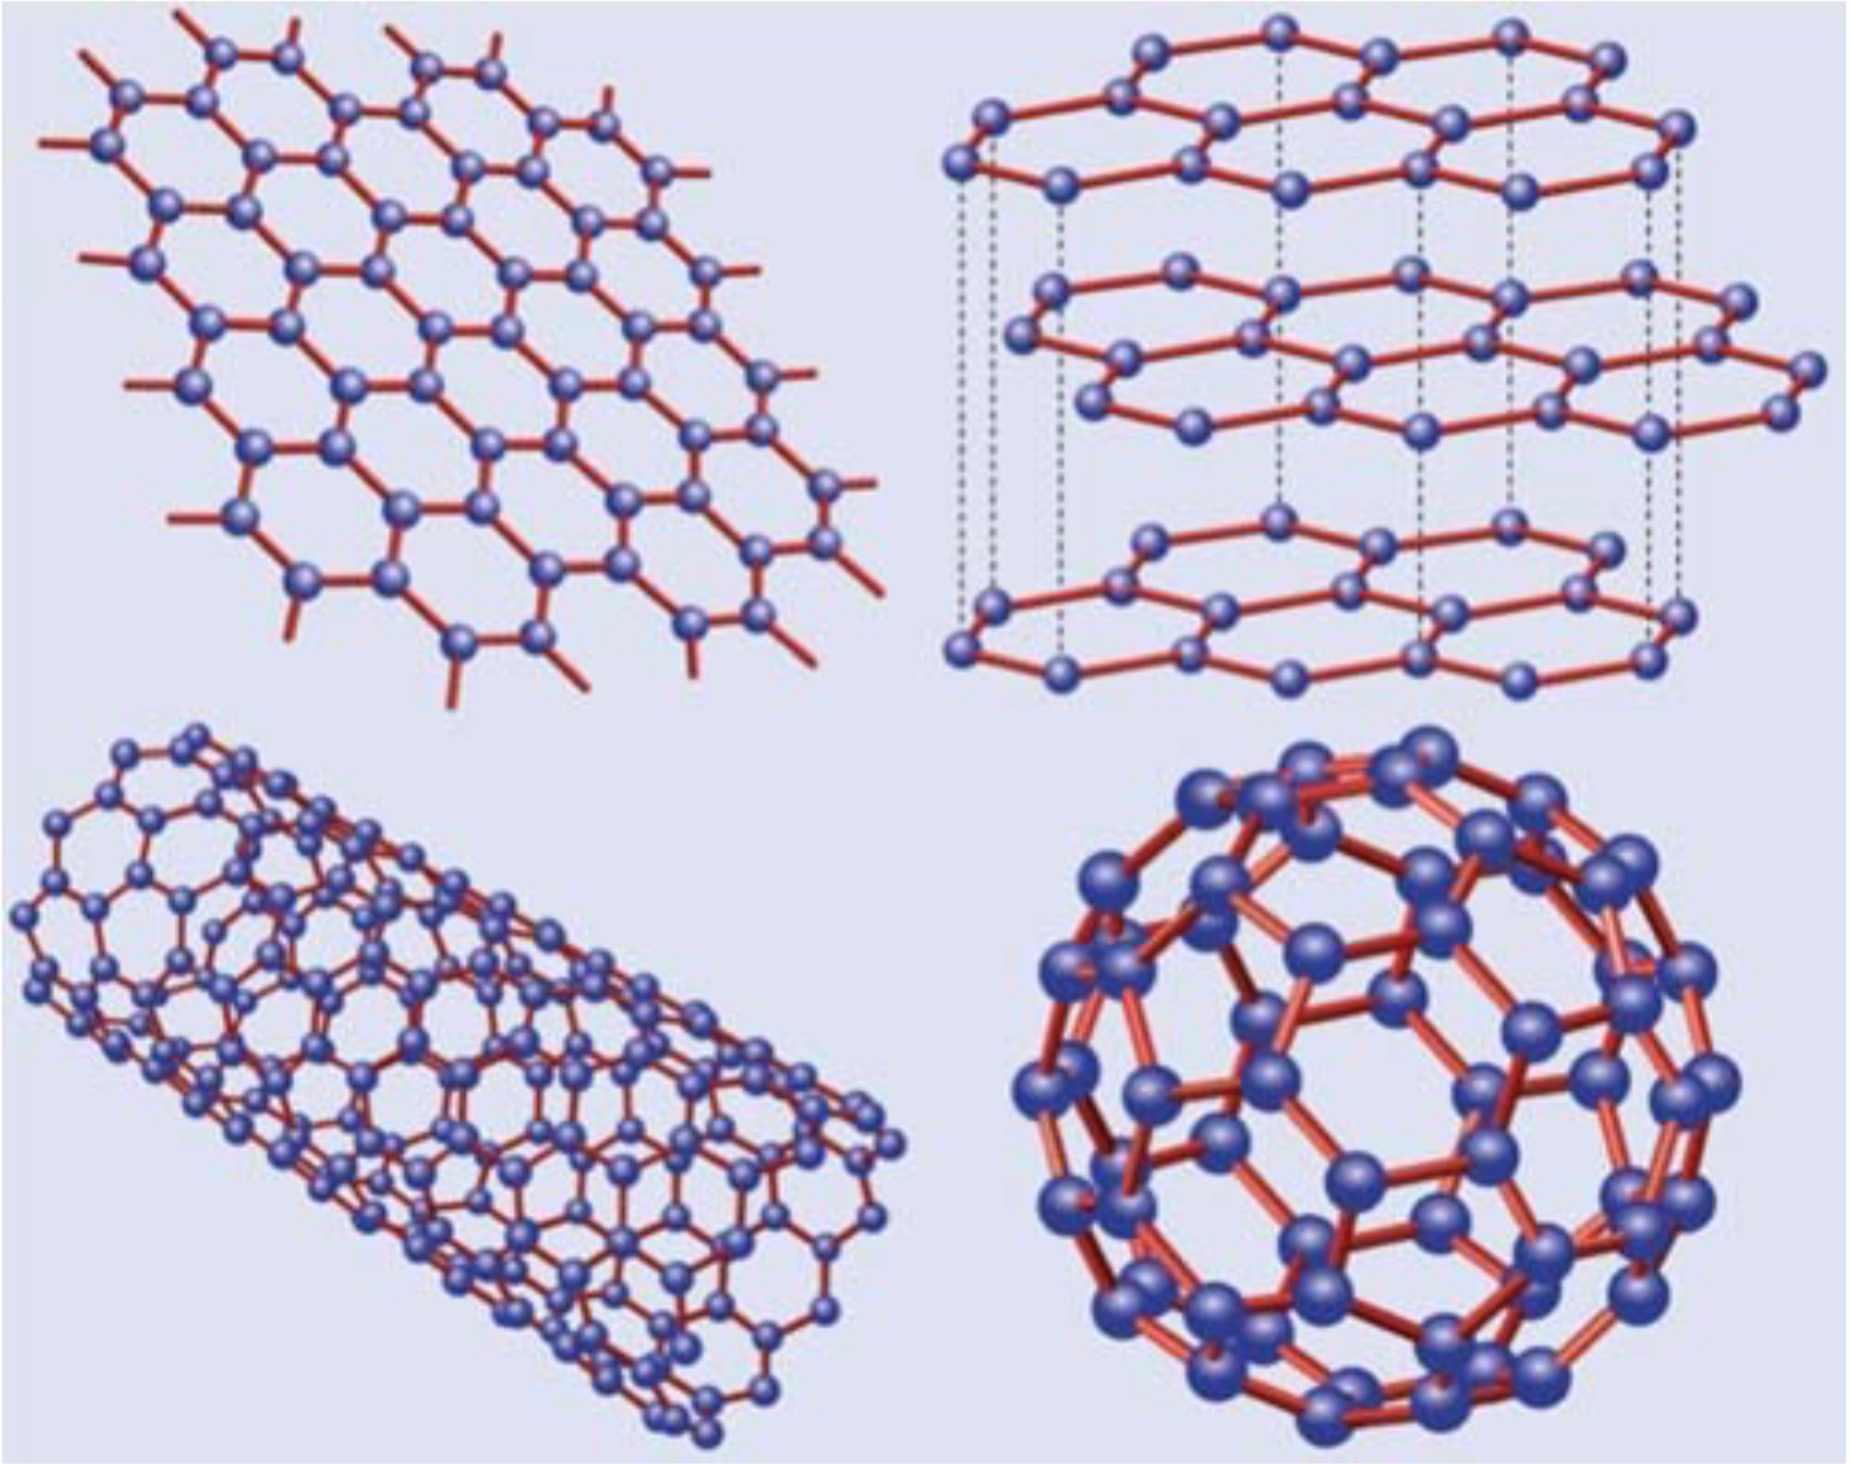
\includegraphics[width=0.38\textwidth]{graphene}
  \caption{Graphical interpretation of the different structures of graphene. Top left shows a graphene monolayer beside a 3-layered graphite structure. Bottom left shows a carbon nanotube beside a $C_{60}$ fullerene.}
  \label{graphene}
\end{wrapfigure}

Carbon, which not only is one of the key elements in every known life form, also has a wide span of applications ranging from common lead in pencils to jewelry in the form of rare earth diamonds. Extensive research has been conducted on graphene, due to the fascinating abilities of this material such as an electron mobility of $2.5 \cdot 10^5$cm$^2$V$^{-1}$s$^{-1}$.\cite{grapheneroad} which is much greater than the mobility in typical metals of 50 cm$^2$V$^{-1}$s$^{-1}$.\cite{mobilitybog} Furthermore the Youngs modulus of graphene has been measured to 1 TPa and the intrinsic strength of 130 Gpa.\cite{grapheneroad} A thermal conductivity exceeding 3,000 W mK$^{-1}$, adds to the remarkeable abilities of graphene.\\

Graphene is a two dimensional honeycomb lattice of carbon atoms. Each carbon atom is $sp^2$ hybridized where one $s$ orbital and two $p$ orbitals form three planar bonds with a separation angle of 120\degree.\cite{RevModPhys.81.109} The distance between the individual carbon atoms is 1.42 Å. Due to the flexibility of the $sp^2$ bonds in the z direction, many other structures can be formed by a sheet of graphene, such as fullerenes, carbon nanotubes, and graphite. Fullerenes are the shape of balls, consisting of 60 carbon atoms. These balls are formed from a wrapped up graphene sheet. The graphene sheet is wrapped up due to the formation of pentagons. Carbon nanotubes has the shape of a tube, naturally, and are formed from the connection of two edges on a graphene sheet. Graphite, at last, is the stucture arising, when multiple layers of graphene are stacked on top of each other. Here the Van Der Waals forces between the individual layers, are the only thing that keeps the layers on top of each other. All of these structures are shown in Figure \ref{graphene}. The graphene unit cell consists of only two lattice points, and the lattice vectors can be written as the following:

\begin{align*}
  a_1 = \frac{a}{2}(3,-\sqrt{3}) \; a_2 = \frac{a}{2}(3,\sqrt{3})
\end{align*}



\section{Graphene on Ir(111)}

As a monolayer of graphene is synthesized on top of a metal surface the underlying metal and the graphene monolayer rarely has identical lattice parameters. This causes a mismatch between the two layers which causes areas were the two layers are perfectly aligned as well as areas where both layers are complete out of phase. This causes a phenomenon known as a moiré effect, where a superstructure appears from the two mismatching patterns.\\
During these experiments, graphene on top of an Ir(111) surface is studied. Ir crystallises as a face centered cubic lattice, and once cut in the [111] direction, the surface atoms have a hexagonal close packed arrangement.\cite{kibler2003preparation} The atomic diameter of Ir is 2.715 Å\cite{kibler2003preparation}, which differs slightly from the graphene lattice with a periodicity of 2.45$\pm$0.04Å \cite{1367-2630-10-4-043033}, and a moiré pattern is therefore expected.\\
Graphene on Ir(111) has a well-defined moiré structure which is depicted in Figure \ref{moire}. Here the grey atoms shows the Ir(111) surface, and the red layer on top corresponds to the graphene sheet. The moiré pattern is seen as bright spots across the surface where an Ir atom is directly below the center of a graphene hexagon. It is seen from Figure \ref{moire} that the moiré pattern has a periodicity, and the repeat vector is found in the literature with a length of 25.2$\pm$0.4Å.\cite{1367-2630-10-4-043033}\\
The graphene on Ir(111) moiré unit cell is outlined in Figure \ref{moire} and a zoom of this is shown in Figure \ref{grirmoire}. In this figure the ATOP, FCC and HCP positions are marked by circles. These areas within the unit cell are of special interest due to special alignments between the underlying Ir(111) atoms and the graphene sheet. The ATOP sites are positioned in the corners of the unit cell rhombus where an Ir atom is just below the center of a graphene hexagon. In these sites the distance to the underlying Ir(111) surface is slightly higher than the FCC and HCP sites, and therefore the sheet resemble free standing graphene.\cite{PhysRevB.93.115403} In the HCP site the graphene hexagon is aligned with the two underlying Ir layers as a HCP lattice. This means that an atom from the Ir(S-1) layer is directly under the center of a graphene hexagon. In the FCC site, an atom from the Ir(S-2) layer is directly under the center of a graphene hexagon. Every second carbon atom is directly above an Ir atom, in both the HCP and FCC site.\cite{voloshina2013electronic}

\begin{figure}[H]
  \centering
  \begin{subfigure}[b]{0.4\textwidth}
       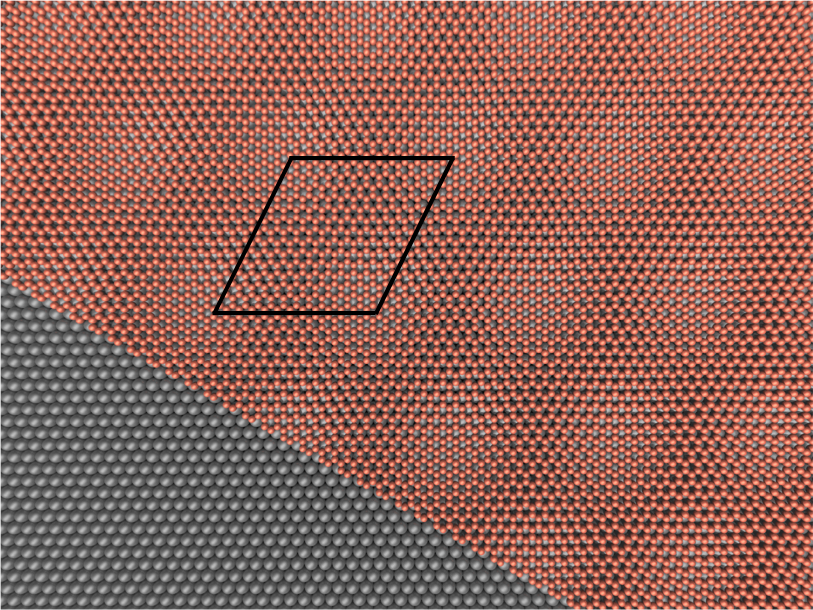
\includegraphics[width=\textwidth]{moire}
       \caption{}
       \label{moire}
   \end{subfigure}
   \begin{subfigure}[b]{0.4\textwidth}
        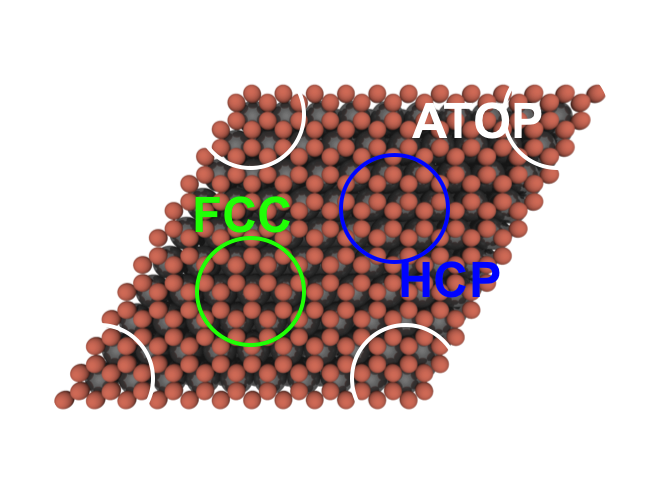
\includegraphics[width=\textwidth]{grirmoire}
        \caption{}
        \label{grirmoire}
    \end{subfigure}
  \caption{Graphical interpretation of graphene on Ir(111). (a) shows a Ir(111) (grey) surface with the moiré structure once the graphene sheet (red) is on top. (b) shows a moiré unit cell. \cite{Line}}
  \label{moireunitcell}
\end{figure}


\section{Hydrogenation of graphene on Ir(111) using atomic deuterium}

The properties of graphene changes drastically with chemical functionalization of different species. The adsorption of any species is highly determined by the underlying surface, which in this study is Ir(111). The adsorption of hydrogen to the Gr/Ir surface is a highly wanted mechanism to understand, due to the special abilities arising from the functionalization of graphene by hydrogen. These effects include a bandgap opening of at least 450meV.\cite{e40134a5a1aa4cb69ba806c02cd8e327} The bandgap opens up for a large number of possibilities for the usage of functionalized graphene, where the most appealing is constructing a new type of field effect transistors. Other forms of applications of functionalized graphene is within energy storage. Due to the one atom thick monolayer it is desirable to use graphene to store hydrogen.\\
As hydrogen is adsorbed to the graphene monolayer, the structural arrangement is changed. Due to the adsorbed hydrogen atom, the graphene undergoes a transition from $sp^2$ hybridization to $sp^3$ hybridization. This implies that the otherwise flat graphene sheet is distorted due to the 3-dimensional conformation of the bonds in the $sp^3$ hybridization. Every second carbon atom is turning downwards and constructs a bond to the underlying Ir(111) surface. This is only possible in the HCP and FCC sites of the moiré unit cell where every second carbon atom of the graphene is directly above an Iridium atom. This induce that the hydrogenation of graphene follows the moiré pattern.\cite{PhysRevB.93.115403} It is therefore expected to observe a superstructure from the hydrogenated surface with the same periodicity as the moiré pattern.\\
A graphical interpretation of the hydrogenation of graphene on Ir(111) is shown in figure \ref{hydrogenation:all}, which is made by Line Kyhl. Here it is seen that clusters of hydrogen bind to the carbon atoms in the FCC and HCP sites. Figure \ref{hydrogenationside} demonstrates how every other carbon atom binds to the Ir(111) surface and every other binds to a hydrogen atom. Furthermore dimers of hydrogen is seen binding to the surface at the ATOP sites. In these regions the distance to the Iridium is increased compared to the FCC and HCP sites. In these areas the graphene resemble free standing sheets and no bonds are formed between the Iridium and the carbon atoms.

\begin{figure}[H]
  \centering
  \begin{subfigure}[b]{0.4\textwidth}
       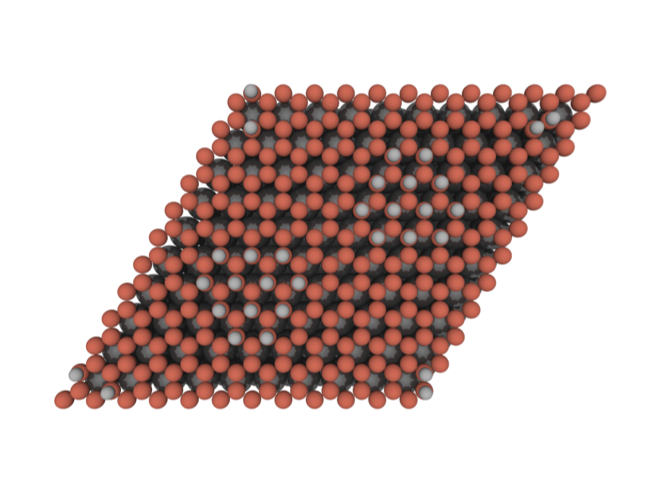
\includegraphics[width=\textwidth]{atomichydrogenation}
       \caption{}
       \label{hydrogenation}
   \end{subfigure}
   \begin{subfigure}[b]{0.4\textwidth}
        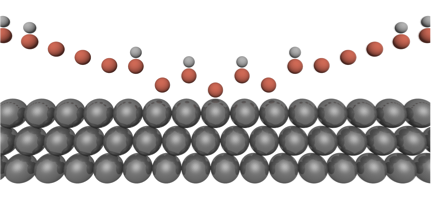
\includegraphics[width=\textwidth]{atomichydrogenationside}
        \caption{}
        \label{hydrogenationside}
    \end{subfigure}
  \caption{Graphical interpretation of the hydrogenation of graphene on Ir(111) by hot atoms.\cite{Line}}
  \label{hydrogenation:all}
\end{figure}



\subsection{Formation of Vibrationally Excited Deuterium}

Vibrationally excited hydrogen molecules have been found to arise from recombinative desorption from metal walls. This happens as atomic hydrogen from a gas phase recombine with hydrogen stuck to the surface. This mechanism produces excited molecules at vibrational states as high as $v'' = 9$.\cite{PhysRevLett.60.337} The vibrational states follow a boltzmann distribution at levels up to $v'' = 3$, and a non boltzmann distribution with an excess off excited states at higher levels. The energy of a hydrogen molecule in the $v'' =9$ state is 3.56 eV, which is enough to dissociate onto free standing graphene with an adsorption barrier ranging from 3.3 eV to 3.9 eV for relaxed graphene, and ranging from 4.3 eV to 4.7 eV for unrelaxed graphene.\cite{:/content/aip/journal/jap/93/6/10.1063/1.1555701}\\
The formation of vibrationally excited molecules is limited by the amount of atomic hydrogen produced. By using a hot filament, it is possible to dissociate hydrogen molecules on the filament surface, and thereby create an atomic gas phase. The coverage on this filament is low once heated and the fraction of a monolayer is in the order of $\theta < 10^{-4}$.\cite{PhysRevLett.60.341} Therefore a valid assumption is that the hydrogen molecules from the gas phase are impinging on a clean surface. From this assumption the flux of atomic hydrogen from the surface is given by:\cite{PhysRevLett.60.341}

\begin{align}
  \phi (H) = 2 s_m P_a \phi (H_2)
\end{align}

Here $s_m$ is the sticking probability of molecular hydrogen and $P_a$ is the atomization probability. $\phi(H_2)$ is the flux of molecular hydrogen towards the surface. The factor of 2 accounts for the two hydrogen atoms resulting from the dissociation of a single molecule. The sticking probability is a material and temperature dependant factor, and the flux of molecules towards the surface is a function of the pressure of the gas phase. The probability of atomization is given by the following:\cite{PhysRevLett.60.341}

\begin{align}
  P_a = \frac{1}{4} [\{(K_p/\gamma p)(K_p / \gamma p + 8)\}^{\frac{1}{2}} -K_p/\gamma p],
\end{align}

where $K_p$ is the equilibrium constant of the atomization reaction, $\gamma = \sqrt{\frac{T_f}{T_g}}$, with subscripts indicating the temperature of the filament and gas respectively. The gas pressure is $p$. During this study the hydrogenation of graphene on Ir(111) is investigated, and the hydrogenation threshold is estimated. By changing the amount of atomic hydrogen impinging the walls in the UHV chamber, the point at which no hydrogen is adsorbed to the graphene on Ir(111) surface can be found. During these experiments the gas pressure as well as the gas temperature is kept constant. Hence the temperature of the hydrogen cracker is altered in order to find the temperature, at which the number of excited molecules, in the high vibrational levels, is close to zero.

%\begin{figure}[H]
%  \centering
%  \begin{subfigure}[b]{0.4\textwidth}
%       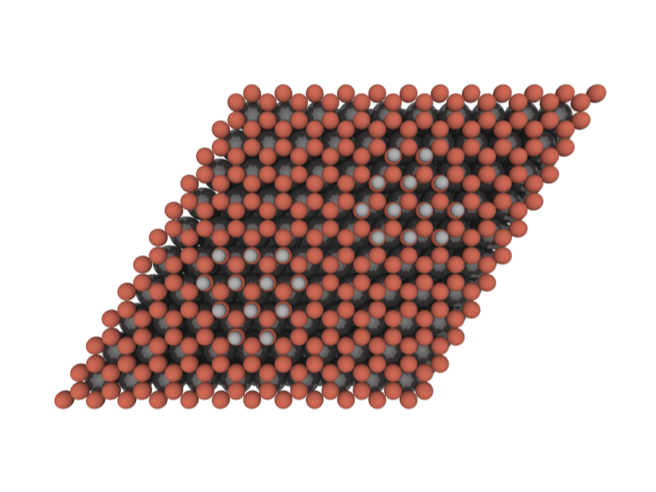
\includegraphics[width=\textwidth]{molecularhydrogenation}
%       \caption{}
%       \label{molhydrogenation}
%   \end{subfigure}
%   \begin{subfigure}[b]{0.4\textwidth}
%        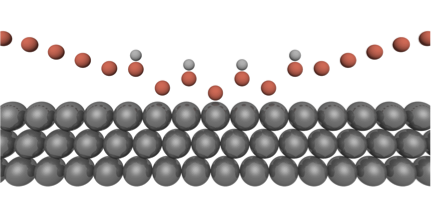
\includegraphics[width=\textwidth]{molecularhydrogenationside}
%        \caption{}
%        \label{molhydrogenationside}
%    \end{subfigure}
%  \caption{Graphical interpretation of the hydrogenation of graphene on Ir(111) by vibrationally excited molecules.\cite{Line}}
%  \label{molhydrogenation:all}
%\end{figure}
